\documentclass[t,xcolor={usenames,dvipsnames}]{beamer}

\mode<presentation>
{
\usetheme{Frankfurt}%{Warsaw}
%\setbeamercovered{transparent}
%\setbeamercolor{background canvas}{bg=white}
}

% Delete these, if you do not want the table of contents to pop up at
% the beginning of each (sub)section:
%\AtBeginSubsection[]
%{
%  \begin{frame}<beamer>{Outline}
%    \tableofcontents[currentsection,currentsubsection]
%  \end{frame}
%}
%\AtBeginSection[]
%{
%  \begin{frame}<beamer>{Outline}
%    \tableofcontents[currentsection]
%  \end{frame}
%}

\usepackage[english]{babel}
\usepackage[latin1]{inputenc}
\usepackage{times}
\usepackage[T1]{fontenc}
\usepackage{verbatim}
\usepackage{url}
\usepackage{amsmath,amssymb}
\usepackage{comment}
\usepackage[overlay,absolute]{textpos}
\usepackage{hyperref}

% Author-date citations
\usepackage[authoryear,round]{natbib}
\let\cite=\citep  % default \cite such as {\LaTeX} authors are used to

% Where \includegraphics should look for figures
\graphicspath{{./figs/}{../group_talk_2011_11_29/figs/}}
\usepackage{epstopdf}
\DeclareGraphicsExtensions{.eps,.png,.jpg,.pdf}

% Shortcuts
\newcommand{\myhref}[2]{\href{#1}{\textcolor{Blue}{#2}}}
\newcommand{\myurl}[1]{\myhref{#1}{#1}}
\newcommand{\subitem}[1]{\begin{itemize}[<.->]\item #1 \end{itemize}}
\newcommand{\ghead}[1]{{\tiny #1\\}}
\newcommand{\doi}[1]{\myhref{http://dx.doi.org/#1}{doi:#1}}
\newcommand{\csym}[1]{\textcolor{Blue}{\texttt{#1}}}
\newcommand{\ud}{\mathrm{d}}
\newcommand{\dt}{\ud t}

%%%%%%%%%%%%%%%%%%%%%%%%%%%%%%%%%%%%%%%%%%%%%%%%%%%%%%%%%%%%%%%%%%%%%%
\title{Functional Curation and Global Ecosystem Modelling}
\author{Jonathan Cooper}
\institute[University of Oxford]
{Computational Biology Group\\
 Department of Computer Science\\
 University of Oxford}
\date{January 14, 2014}

\begin{document}

\begin{frame}
\titlepage
\end{frame}

%%%%%%%%%%%%%%%%%%%%%%%%%%%%%%%%%%%%%%%%%%%%%%%%%%%%%%%%%%%%%%%%%%%%%%

%\begin{frame}{Outline}
%\setcounter{tocdepth}{1}
%\tableofcontents
%\end{frame}

%%%%%%%%%%%%%%%%%%%%%%%%%%%%%%%%%%%%%%%%%%%%%%%%%%%%%%%%%%%%%%%%%%%%%%
\section{Motivation}
\subsection*{Main}
%%%%%%%%%%%%%%%%%%%%%%%%%%%%%%%%%%%%%%%%%%%%%%%%%%%%%%%%%%%%%%%%%%%%%%

\begin{frame}{(Re)Using models}
\begin{itemize}
\item As hypothesis encodings, models are developed \emph{for a specific purpose}
  \subitem{May not be appropriate for studying the same system in a different context}
\item How can we\ldots
  \begin{itemize}
  \item determine a model's functionality, i.e.\ its suitability or limitations for a new study?
  \item re-use a model in a different experimental context?
  \item compare hypotheses: different models' behaviours under the same experiment?
  \end{itemize}
\end{itemize}
\end{frame}


%%%%%%%%%%%%%%%%%%%%%%%%%%%%%%%%%%%%%%%%%%%%%%%%%%%%%%%%%%%%%%%%%%%%%%
\section{Functional curation with virtual experiments}
\subsection*{Main}
%%%%%%%%%%%%%%%%%%%%%%%%%%%%%%%%%%%%%%%%%%%%%%%%%%%%%%%%%%%%%%%%%%%%%%

\begin{frame}{The essence of Functional Curation}
\subitem{Separate \alert{model structure} and \alert{experimental scenario}}
\begin{center}
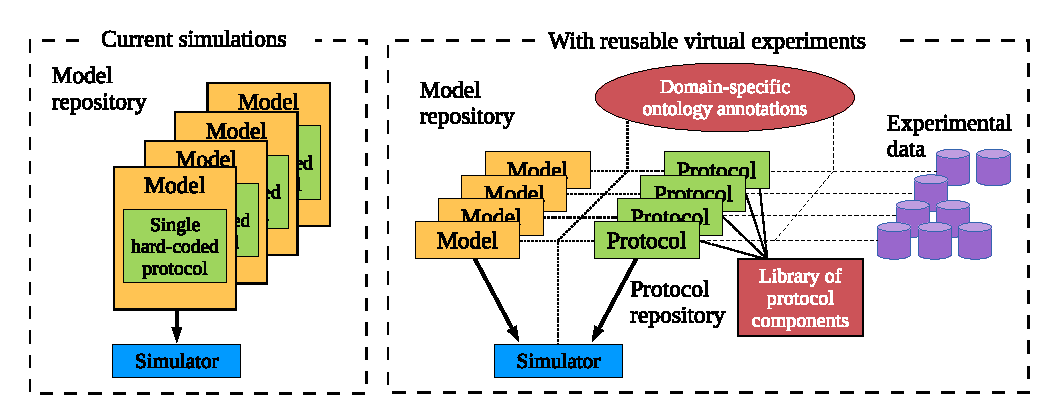
\includegraphics[width=.9\textwidth]{VirtEx_new}
\end{center}
\vspace{-.25cm}
\begin{itemize}
\item Apply any \alert{virtual experiment} to any (relevant) model
\item One definitive version of each model / protocol
\item Automatically generate post-processed outputs, plots, etc.
\end{itemize}
\end{frame}


%%%%%%%%%%%%%%%%%%%%%%%%%%%%%%%%%%%%%%%%%%%%%%%%%%%%%%%%%%%%%%%%%%%%%%
\section{Examples}
%%%%%%%%%%%%%%%%%%%%%%%%%%%%%%%%%%%%%%%%%%%%%%%%%%%%%%%%%%%%%%%%%%%%%%

\begin{frame}{Initial application: cardiac electrophysiology}
\small
Suppose we have our mathematical model, e.g.\ Hund \& Rudy 2004:\\
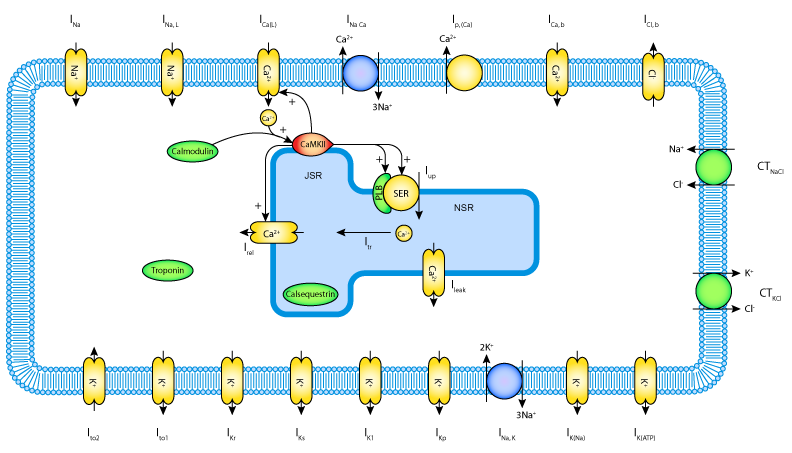
\includegraphics[width=\textwidth]{hund_2004}\\
We want to perform various potentially complex interventions\ldots
\end{frame}

\subsection*{S1-S2}
%%%%%%%%%%%%%%%%%%%

\begin{frame}{Example: S1-S2 restitution}
\begin{center}
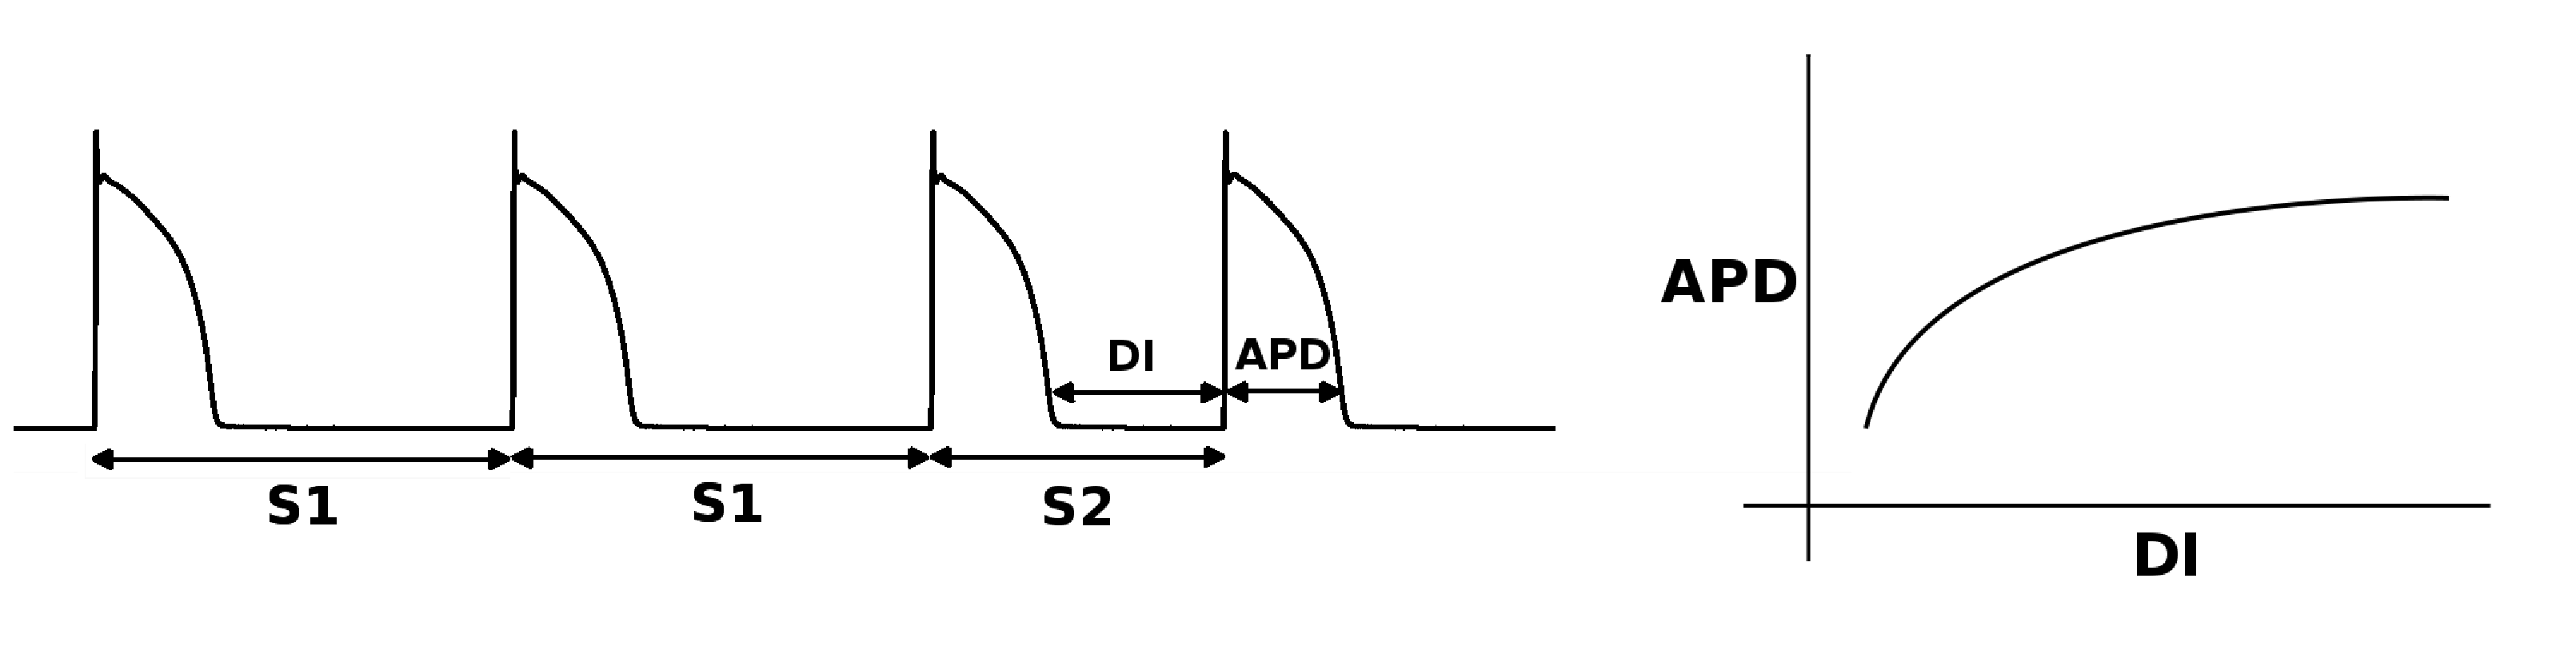
\includegraphics[width=\textwidth]{S1S2}
\end{center}
\end{frame}

\begin{frame}{Example: S1-S2 restitution on canine models}
\begin{columns}[T]
\begin{column}{.33\linewidth}
\begin{center}
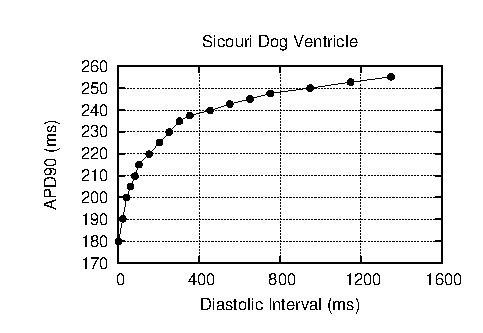
\includegraphics[width=\textwidth]{sicouri_dog_ventricle_s1s2_curve}\\
\vspace{.1cm}
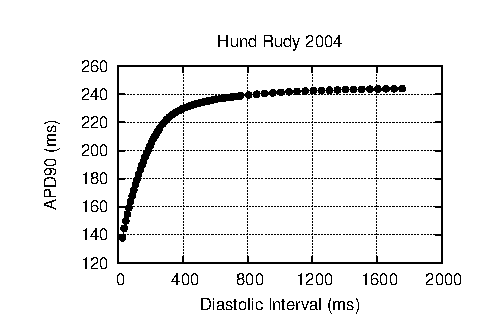
\includegraphics[width=\textwidth]{hund_rudy_2004_s1s2_curve}
\end{center}
\end{column}
\begin{column}{.33\linewidth}
\begin{center}
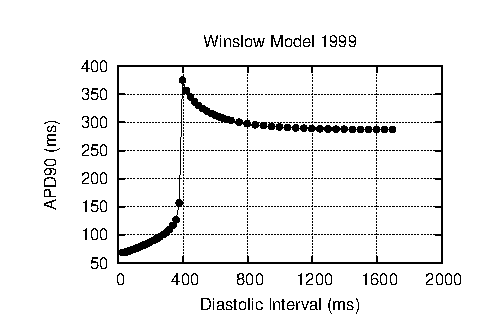
\includegraphics[width=\textwidth]{winslow_model_1999_s1s2_curve}\\
\vspace{.1cm}
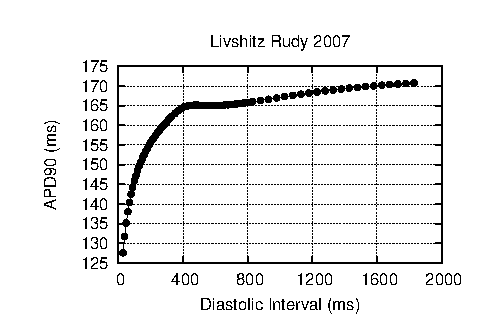
\includegraphics[width=\textwidth]{livshitz_rudy_2007_s1s2_curve}
\end{center}
\end{column}
\begin{column}{.33\linewidth}
\begin{center}
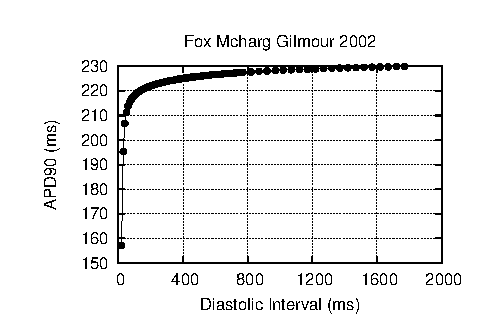
\includegraphics[width=\textwidth]{fox_mcharg_gilmour_2002_s1s2_curve}\\
\vspace{.1cm}
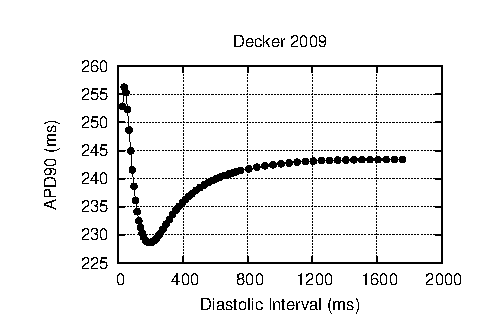
\includegraphics[width=\textwidth]{decker_2009_s1s2_curve}
\end{center}
\end{column}
\end{columns}
\end{frame}

\subsection*{ICaL}
%%%%%%%%%%%%%%%%%%

\begin{frame}{Example: $I_{\textrm{Ca}_L}$ voltage clamp}
\begin{center}
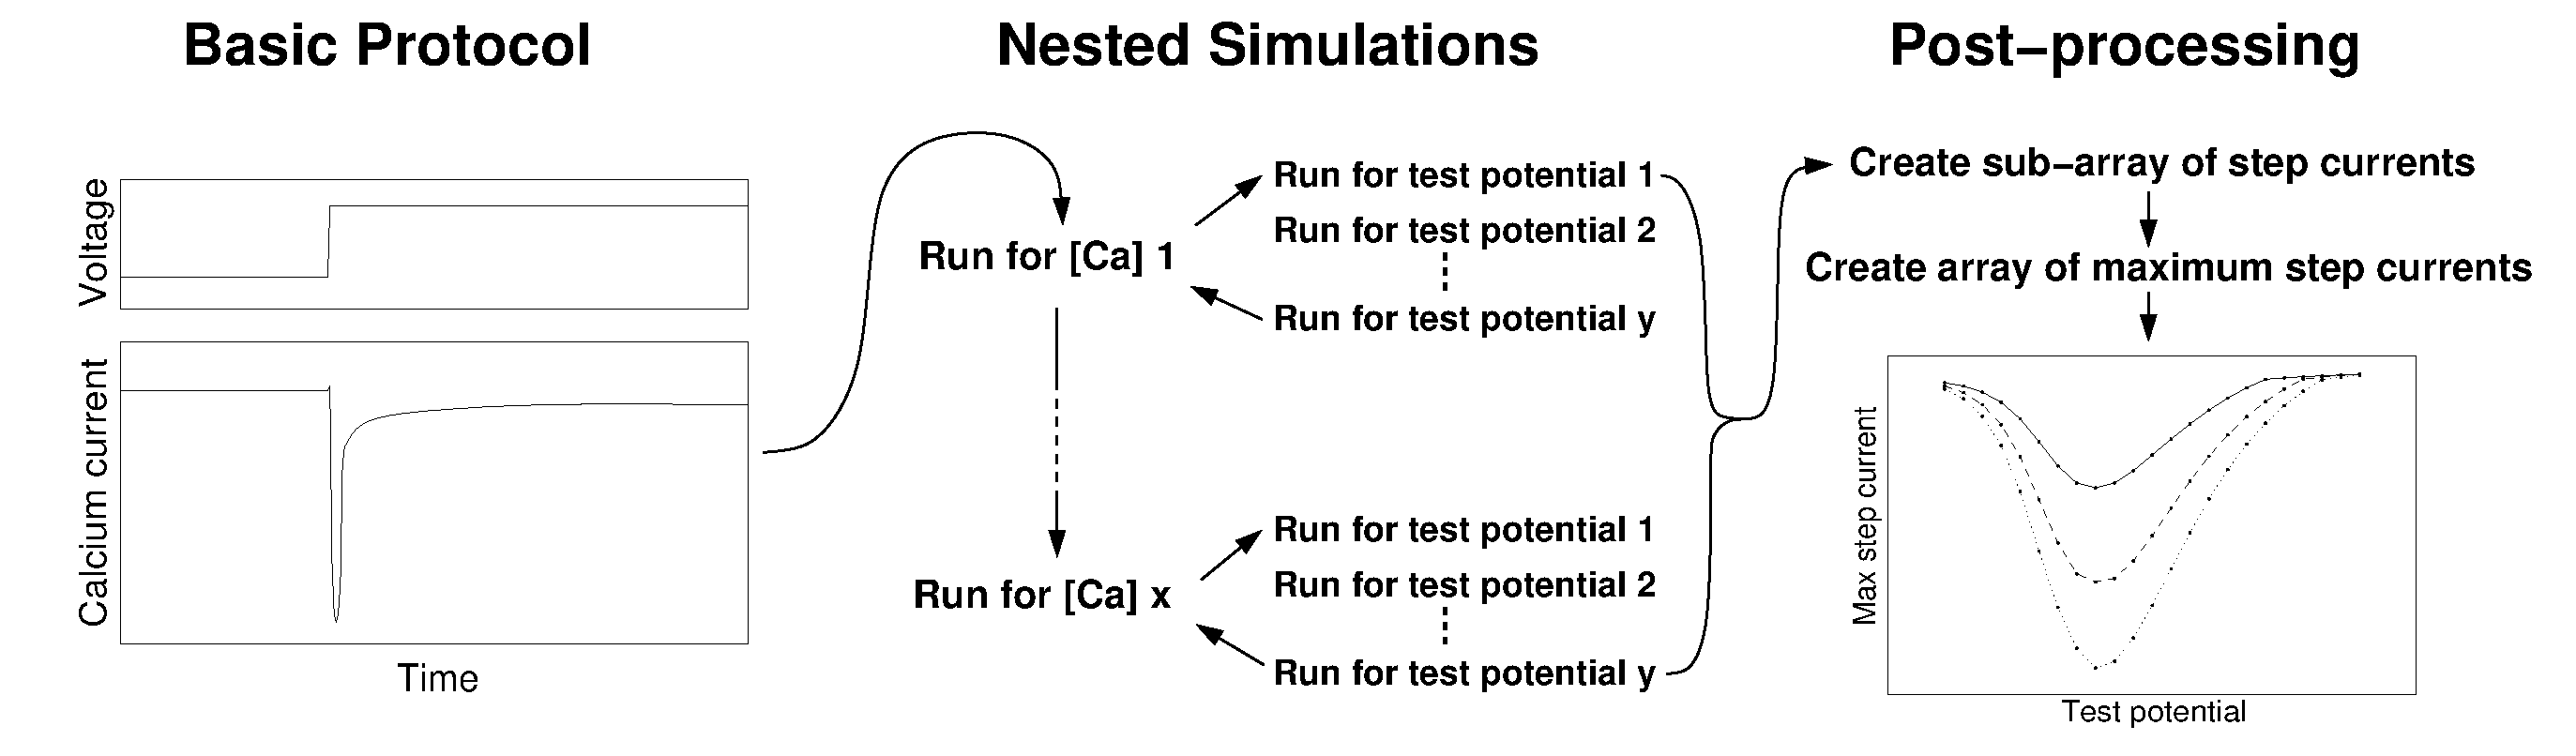
\includegraphics[width=\textwidth]{ICaLIntro}
\end{center}
\end{frame}

\begin{frame}{Example: $I_{\textrm{Ca}_L}$ voltage clamp}
\begin{columns}[T]
\begin{column}{.33\linewidth}
\begin{center}
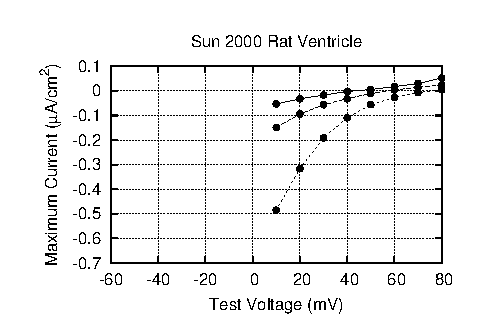
\includegraphics[width=\textwidth]{sun_rat_ventricle_ICaL_IV_curve}\\
\vspace{.1cm}
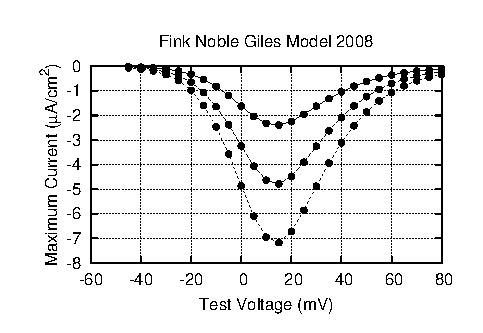
\includegraphics[width=\textwidth]{fink_noble_giles_model_2008_ICaL_IV_curve}
\end{center}
\end{column}
\begin{column}{.33\linewidth}
\begin{center}
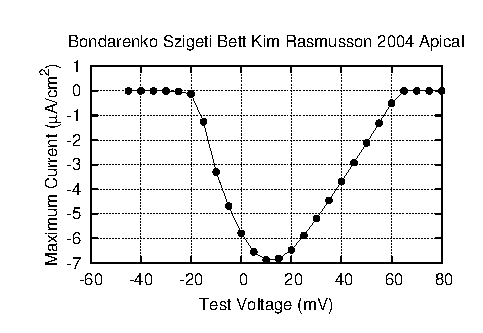
\includegraphics[width=\textwidth]{bondarenko_szigeti_bett_kim_rasmusson_2004_apical_ICaL_IV_curve}\\
\vspace{.1cm}
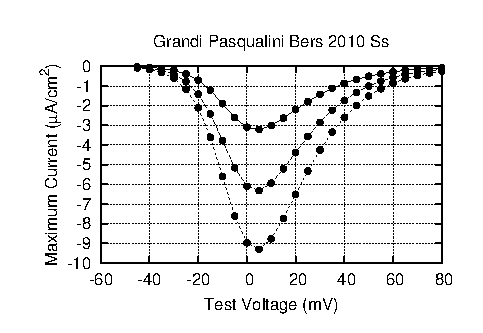
\includegraphics[width=\textwidth]{grandi_pasqualini_bers_2010_ss_ICaL_IV_curve}
\end{center}
\end{column}
\begin{column}{.33\linewidth}
\begin{center}
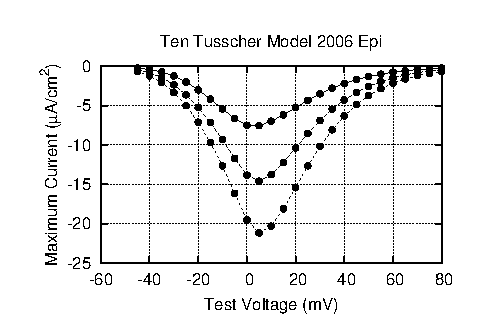
\includegraphics[width=\textwidth]{ten_tusscher_model_2006_epi_ICaL_IV_curve}\\
\vspace{.1cm}
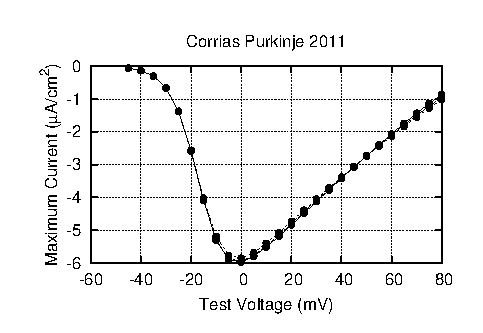
\includegraphics[width=\textwidth]{corrias_purkinje_2011_ICaL_IV_curve}
\end{center}
\end{column}
\end{columns}
\end{frame}
% Refer back to Gary's talk and IC50 calculation


\subsection*{Cell-based Chaste}
%%%%%%%%%%%%%%%%%%%%%%%%%%%%%%%

\begin{frame}{Intestinal crypts}
\begin{itemize}
\item Here a `model' is a cell-based \alert{simulation}, not just equations
  \subitem{Implemented using the cell-based functionality in Chaste}
\item Model parameters may be set
\item Execution may be nested in outer loops, e.g.\ for parameter sweep
\item Result post-processing may be performed
\end{itemize}
\end{frame}


\begin{frame}{Case study}
\centering
\begin{minipage}{0.28\textwidth}
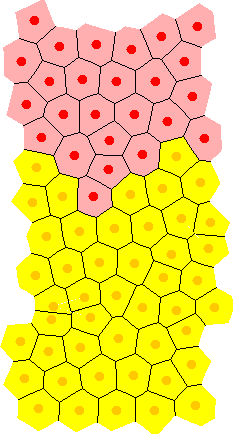
\includegraphics[width=.9\textwidth]{VariableWnt}
\end{minipage}
\begin{minipage}{0.39\textwidth}
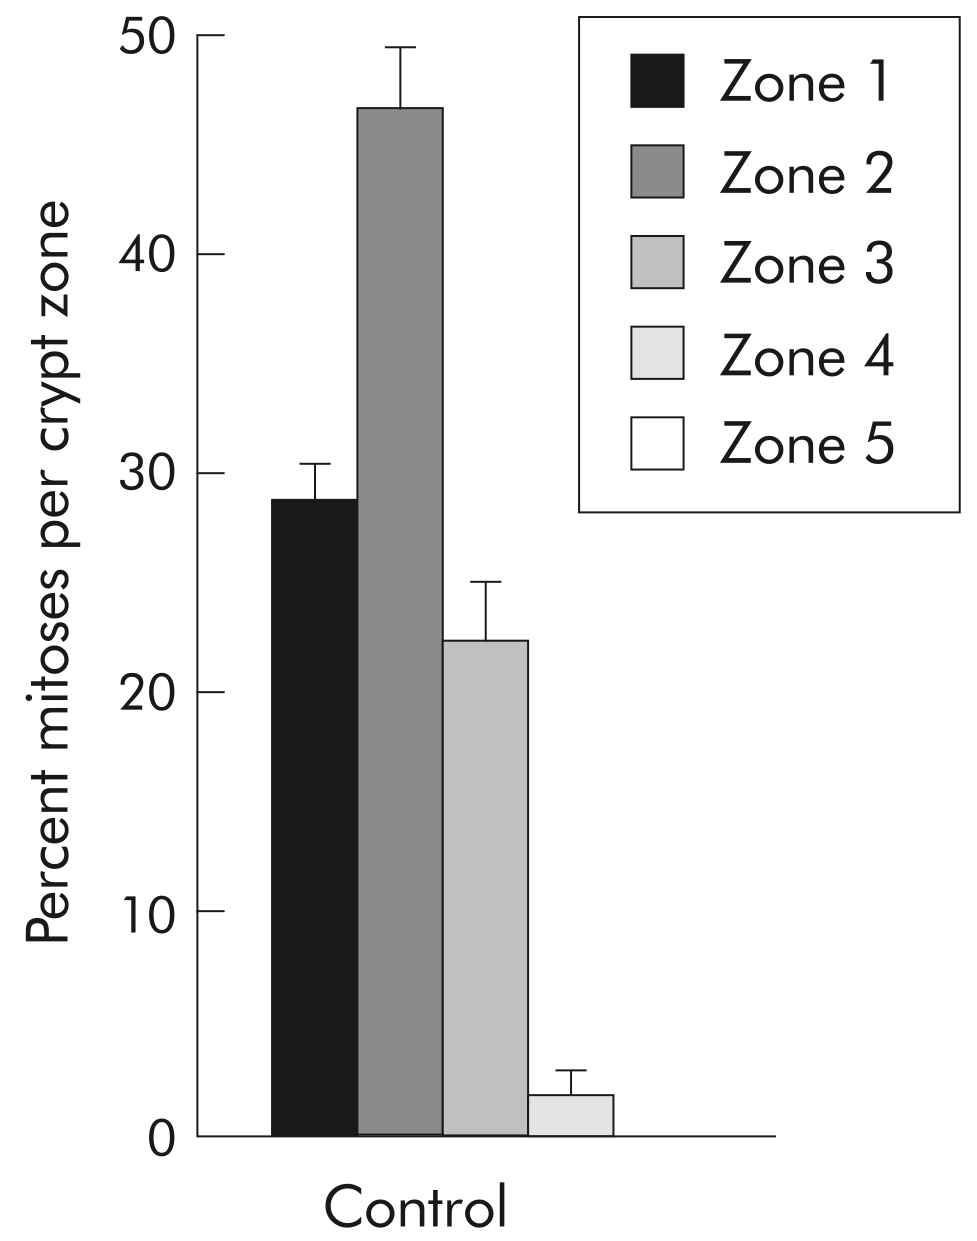
\includegraphics[width=.9\textwidth]{WongFigure}
\end{minipage}
\begin{minipage}{0.31\textwidth}
\begin{itemize}
\item Cell division locations in intestinal crypt
\item Compare three submodels for cell cycle
\item Parameter sweep over crypt height
\end{itemize}
\end{minipage}
\vspace{.4cm}
\begin{center}
\tiny
\myhref{http://dx.doi.org/10.1016/j.procs.2013.05.235}{Cooper and Osborne, ICCS 2013}
\end{center}
\end{frame}


\begin{frame}{Results}
\vspace{-.45cm}
{\footnotesize Distributions of crypt cell division events with different cell cycle models}
\vspace{-.1cm}
\hspace*{2mm}
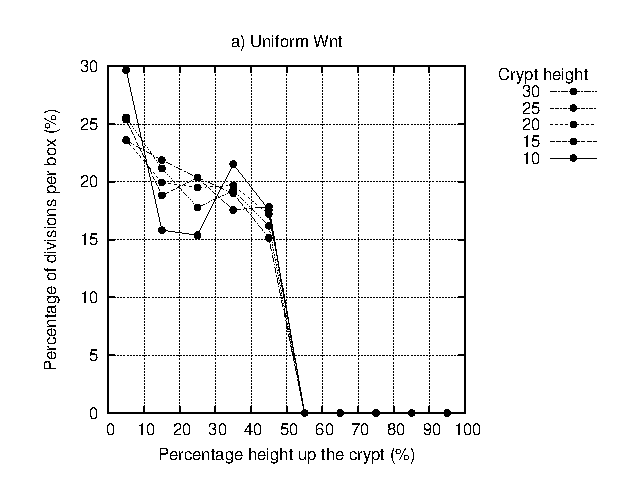
\includegraphics[width=.45\textwidth]{Uniform_Wnt-Cell_division_locations}
\hspace*{5mm}
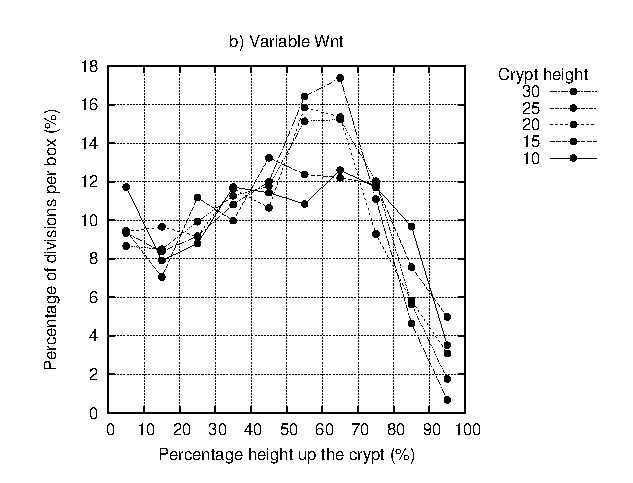
\includegraphics[width=.45\textwidth]{Variable_Wnt-Cell_division_locations}\\
\hspace*{2mm}
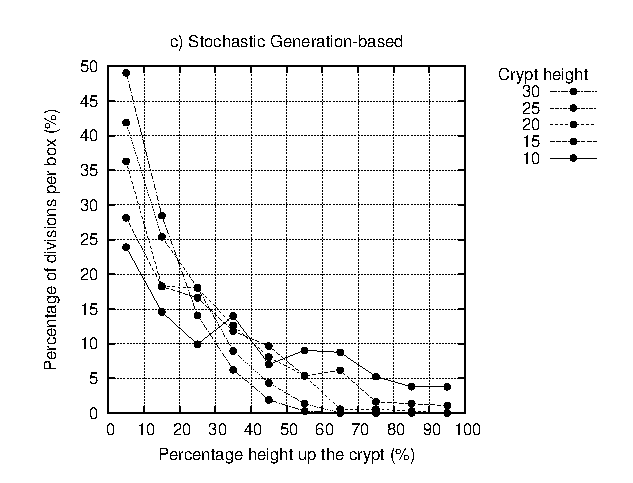
\includegraphics[width=.45\textwidth]{Stochastic_Generation-based-Cell_division_locations}
\hspace*{12mm}
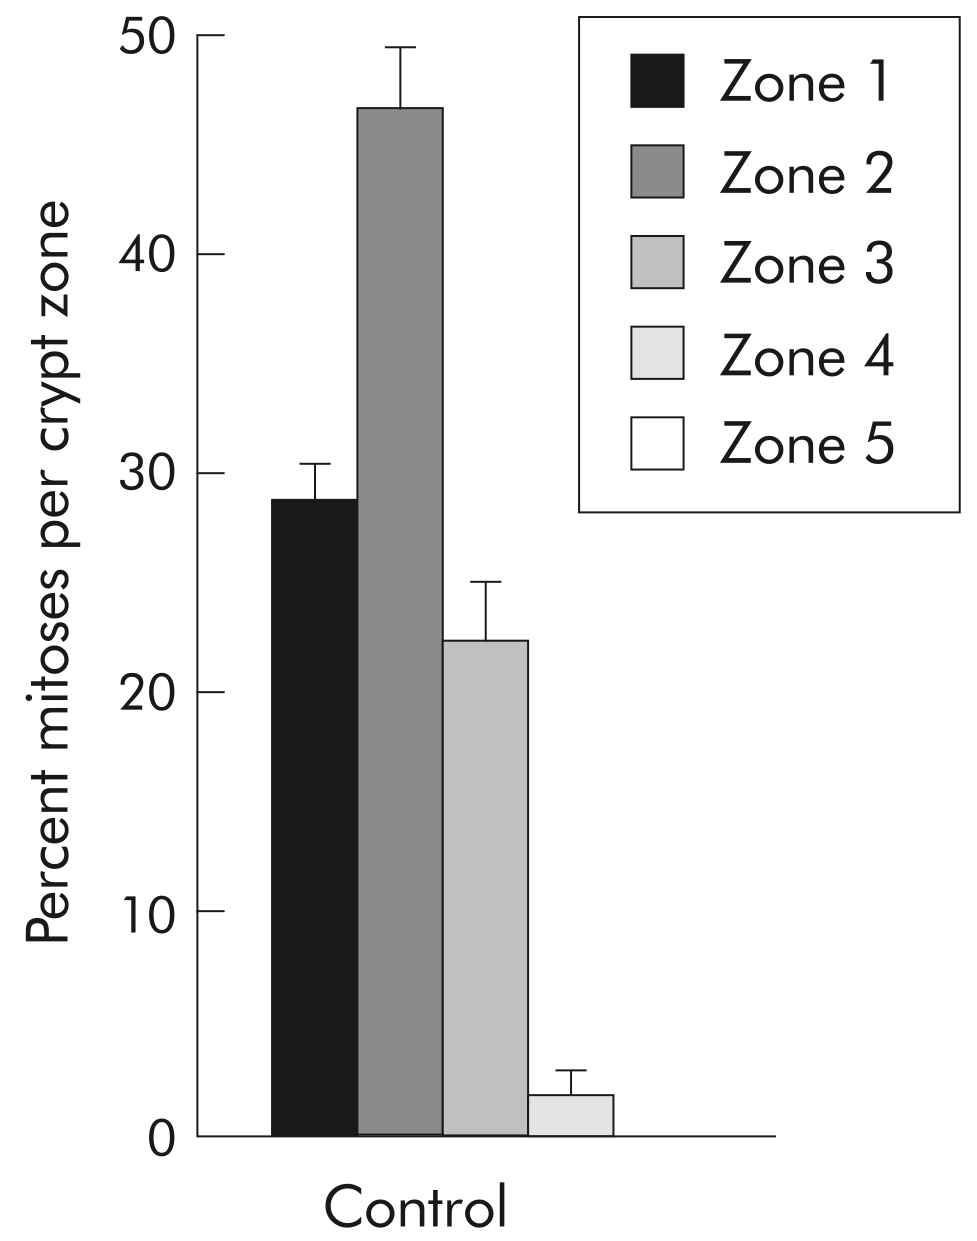
\includegraphics[height=.4\textheight]{WongFigure}
\end{frame}


%%%%%%%%%%%%%%%%%%%%%%%%%%%%%%%%%%%%%%%%%%%%%%%%%%%%%%%%%%%%%%%%%%%%%%
\section{Conclusions and future directions}
\subsection*{Main}
%%%%%%%%%%%%%%%%%%%%%%%%%%%%%%%%%%%%%%%%%%%%%%%%%%%%%%%%%%%%%%%%%%%%%%

\begin{frame}{Goals of this work}
\begin{itemize}
\item Provide a framework for a coherent approach to model fitting, simulation, comparison and validation
  \begin{itemize}
  \item Continuous evaluation of model predictions against experimental data, throughout model lifecycle
  \item Models that are robust, well tested, and well characterised for particular biological studies
  \item Model development akin to high quality software
  \item Improve model reuse \& simulation result reproducibility
  \end{itemize}
\item A functional curation system for each domain
  \begin{itemize}
  \item Brings together competing models, experimental data, and virtual experiments
  \item New models, experiments, or data analysed automatically under all relevant combinations
  \end{itemize}
\end{itemize}
\end{frame}


\begin{frame}{Plans for this year}
\begin{itemize}
\item Comprehensive cardiac protocol suite and website under development
  \subitem{\myurl{https://chaste.cs.ox.ac.uk/FunctionalCuration}}
\item Parameter fitting (with new student Aidan)
  \subitem{Virtual experiments provide simulated data that is directly commensurable, thus providing the objective function to optimise}
\item Developing community standards for virtual experiments (SED-ML)
\item New more flexible implementation using Python
\item Other application domains, notably ecology
  \begin{itemize}
  \item Madingley model (see slide set from Chris McEwen)
  \item Species distribution modelling
  \end{itemize}
\end{itemize}
\end{frame}


\begin{frame}{Madingley model}
\begin{itemize}
\item Aim: clarify what the Madingley model \emph{is}
  \begin{itemize}
  \item Make it easy to change definition of processes, functional groups, etc.
  \item Make it easy to run different experiments
  \end{itemize}
\item Currently: developing a DSL embedded into F\#
  \begin{itemize}
  \item Declare \alert{traits} (e.g.\ `feeding mode'), \alert{functional groups}, and \alert{processes} (e.g.\ `predation')
  \item Implementation based on new version of BME
  \end{itemize}
\item Various pending issues
  \begin{itemize}
  \item Semantics and solvers
  \item Derivation of cohort functions from individualistic descriptions
  \item Interaction with data sources
  \item Spatial behaviour
  \item External DSL syntax
  \end{itemize}
\end{itemize}
\end{frame}


%%%%%%%%%%%%%%%%%%%%%%%%%%%%%%%%%%%%%%%%%%%%%%%%%%%%%%%%%%%%%%%%%%%%%%
\begin{frame}{Acknowledgments}
Gary Mirams, Erich Kerekes, Aidan Daly\\
Chaste team\\
Alan Garny, Steven Niederer, David Gavaghan

Reference publication: \doi{10.1016/j.pbiomolbio.2011.06.003}\\
Website: \myurl{https://chaste.cs.ox.ac.uk/trac/wiki/FunctionalCuration}

\begin{center}

\includegraphics[scale=.9]{chaste-266x60}\\ \vspace{.3cm}

\includegraphics[scale=.7]{logo2020science}\\ \vspace{.4cm}

\includegraphics[width=.55\textwidth]{EPSRC1RGBLO} \hspace{.1cm}

\includegraphics[scale=.55]{logo_msr}
\end{center}
\end{frame}


%%%%%%%%%%%%%%%%%%%%%%%%%%%%%%%%%%%%%%%%%%%%%%%%%%%%%%%%%%%%%%%%%%%%%%
\appendix

\begin{frame}{What goes in a protocol?}
\begin{itemize}
\item Definition of the interface with the model being experimented on
  \begin{itemize}
  \item Handle variations in modelling conventions: naming, encoding the biology in mathematics
  \item Isolate sub-models, using inputs \& outputs of interest
  \end{itemize}
\item Definition of simulations to perform
\item Post-processing operations on simulation results
\item Description of what to plot
\end{itemize}
\end{frame}


\begin{frame}{Our protocol structure}
\begin{center}
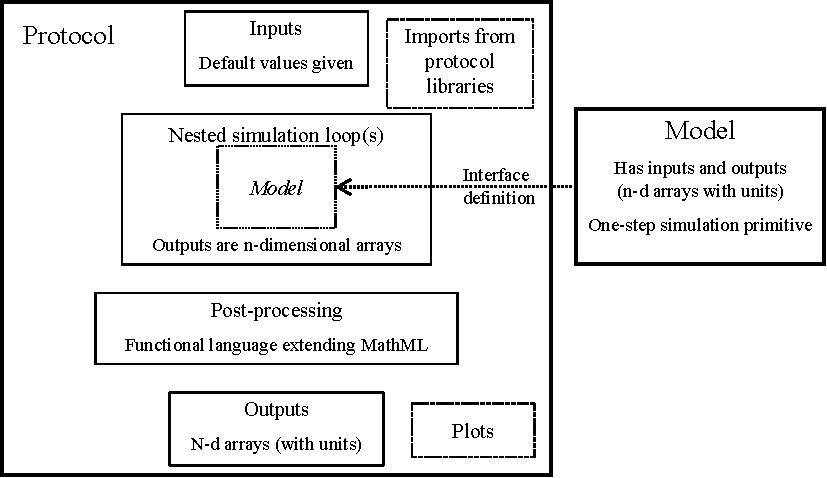
\includegraphics[width=\textwidth]{protocol_language}
\end{center}
\end{frame}


\begin{frame}{Challenges arising from crypt example}
\begin{itemize}
\item Setting `biological' parameters that don't have direct representations in all models
\item Describing the coupling of component models
\item Cell birth \& death imply non-regular result arrays
  \subitem{Increases technical complexity of post-processing}
\item What post-processing should be in the protocol language?
  \begin{itemize}[<.->]
  \item What is best as dedicated code or workflow?
  \item A language targeted at protocol exchange should be supportable by multiple tools
  \item Contrast: rapid prototyping, or deposition in a repository of standard experiments
  \end{itemize}
\end{itemize}
\end{frame}


\begin{frame}{Foundations: a mosaic of standards}
\begin{center}
\includegraphics<1->[scale=.5]{standards_mosaic}\\
{\tiny Fig.: Mosaic of standards, adapted from (\textit{Chelliah et al., 2009, DILS})}
\end{center}
\end{frame}

\begin{frame}{Foundations: a mosaic of standards}
\begin{center}
\includegraphics<1->[scale=.5]{standards_mosaic}\\
{\tiny Fig.: Mosaic of standards, adapted from (\textit{Chelliah et al., 2009, DILS})}
\end{center}
\TPGrid{2}{2}
\begin{textblock}{2}[0.5,0.5](1,1.2)
\centering

\includegraphics[scale=.8]{COMBINE}
\end{textblock}
\end{frame}


\begin{frame}{Simulation Experiment Description Markup Language}
\begin{center}
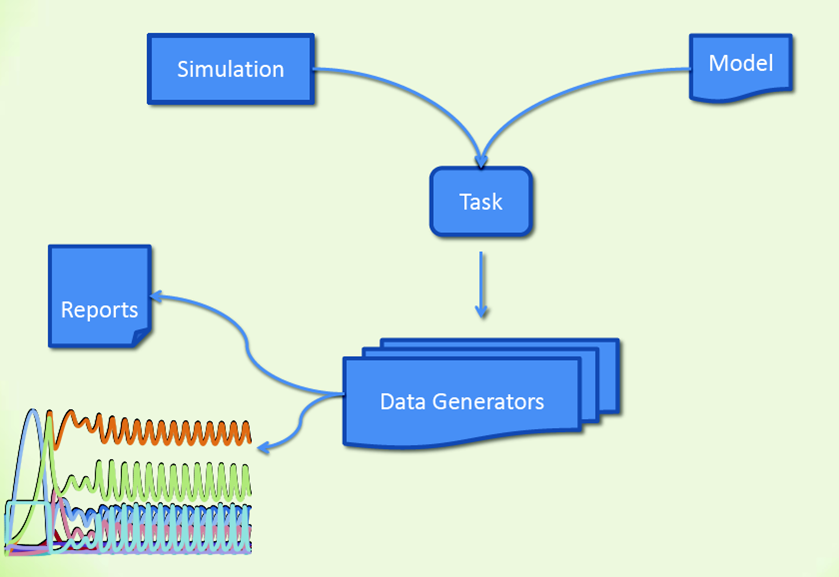
\includegraphics[scale=.5]{SEDML_overview}\\
{\tiny Fig.: SED-ML structure. \textit{Waltemath et al., BMC Sys Biol (2011)}}
\end{center}
\end{frame}

\end{document}
